\chapter{Theorie}
\section{Ruhelage}
Befestigt man das obere Ende einer Feder und hängt an des untere Ende ein Massestück der Masse $m$, so dehnt sich die Feder aus, bis sich ein Kräftegleichgewicht zwischen der Gewichtskraft des Massestücks $F_G$ und der entgegengesetzten Kraft der Feder (Federkraft $F_F$) einstellt. Das Massestück liegt dann in der Ruhelage.
$$F_G = F_R $$

Vernachlässigt man die Masse der Feder, so gilt gemäß dem Hook'schen Gesetz für die Federkraft:
$$F_R = D \cdot s$$
$D$ ist dabei die Federhärte der Feder.
$s$ ist die Auslenkung der Feder. Die Auslenkung ist die Differenz zwischen der Länge, die die Feder hat, wenn keine Kraft auf sie wirkt und der Länge, die sie unter der Krafteinwirkung hat.

In der Ruhelage ist die Feder um eine gewisse Länge, $s_0$ ausgelenkt.

\begin{figure}[H]
\centering
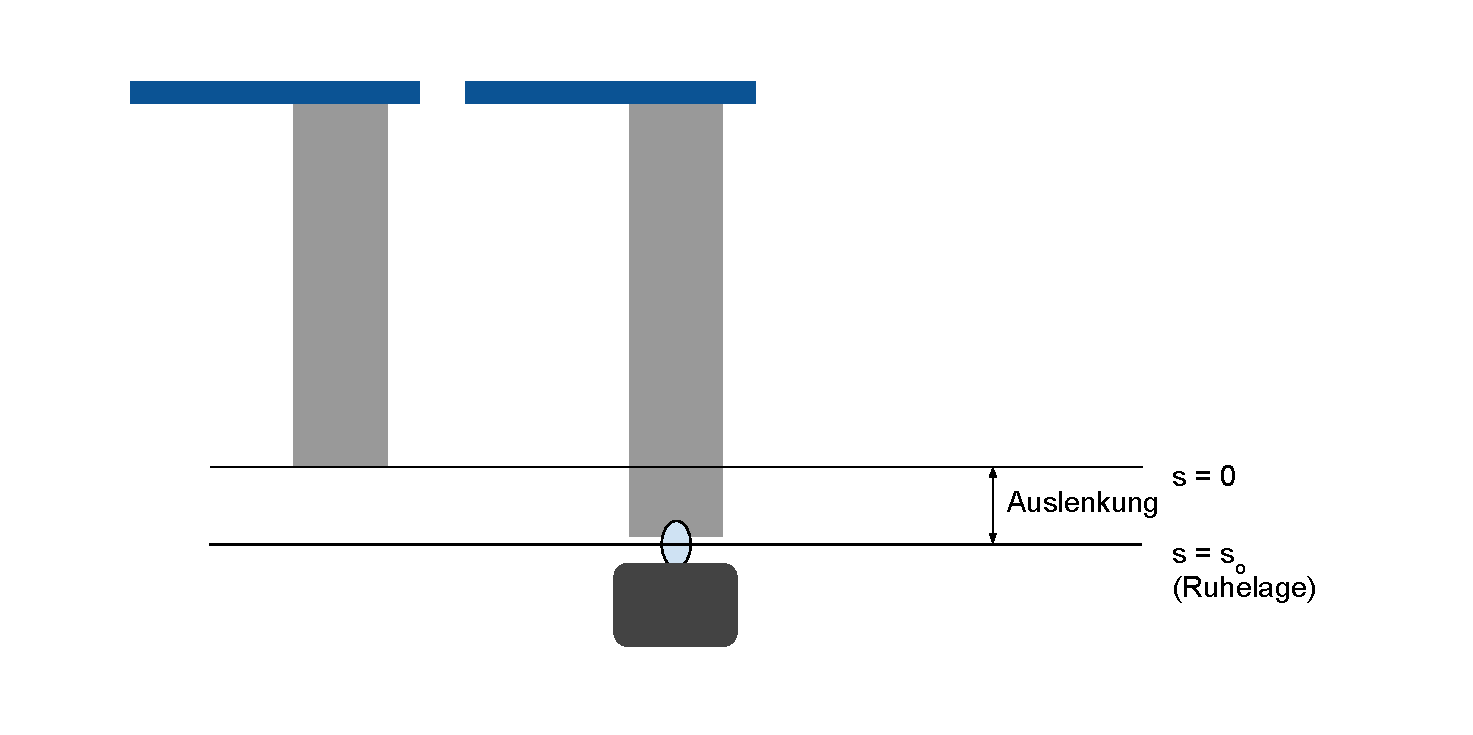
\includegraphics[width=\textwidth]{img/ruhelage.pdf}
\caption{Ruhelage am Federschwerependel}
\end{figure}

\section{Lineares Kraftgesetz}
Wird das Massestück aus der Ruhelage heraus ausgelenkt, wirkt nach dem Hook'schen Gesetz eine entsprechend höhere Federkraft. Die Gewichtskraft bleibt unverändert.
$$F_{F2} = D \cdot (s_0 + s)$$

Zusammen mit der Gewichtskraft des Massestücks ergibt sich als Resultierende Kraft die Rückstellkraft $F_R$ auf das Massestück.
\begin{align*}
F_R &= F_{F2} - F_G \\
F_G &= F_F \\
    &= D \cdot s_0 \\
F_R &= D \cdot (s_0 + s) - D \cdot s_0 \\
    &= D \cdot s
\end{align*}

Da die Rückstellkraft in die entgegengesetzte Richtung der Elongation (Auslenkung aus der Ruhelage) zeigt und in der obigen Herleitung jeweils mit dem Betrag der Kraft gerechnet wurde, muss das Vorzeichen der Rückstellkraft noch umgedreht werden.

$$F_R = -D \cdot s$$

Da die Rückstellkraft einem linearen Kraftgesetz folgt, also proportional zur Elongation ist ($F_R \sim s$), folgt das Federpendel einer harmonischen Schwingung.

\section{Bewegungsgleichung}
Es soll eine Bewegungsgleichung für das schwingende System hergeleitet werden.

Für die Rückstellkraft $F_R$ gilt:
$$F_R = m \cdot a$$

Dabei ist $m$ die Masse des gesamten schwingenden Systems, also das Massestück, sowie Teile der Feder. Letztere wird jedoch vernachlässigt, also ist $m$ die Masse des Massestücks.

Setzt man obige Gleichung in das lineare Kraftgesetz ein, erhält man die Differenzialgleichung der harmonischen Schwingung.
\begin{align*}
m \cdot a &= -D \cdot s \\
m \cdot \ddot s &= -D \cdot s \\
\ddot s &= -\frac{D}{m} \cdot s
\end{align*}

Die allgemeine Lösung für diese Differenzialgleichung ist:

\begin{align*}
s(t) &= \hat s \cdot sin(\omega \cdot t + \varphi_0) \\
\text{mit } \omega &= \sqrt{\frac{D}{m}}
\end{align*}
$\hat s$ ist die maximale Auslenkung aus der Ruhelage, $\varphi$ ist von der Position des Pendels zum Zeitpunkt $t = \SI{0}{\second}$ abhängig.

\section{Periodendauer der Schwingung}
Aus der Kreisfrequenz $\omega$ folgt die Periodendauer $T$:
\begin{align*}
T &= \frac{2\pi}{\omega} \\
  &= \frac{2\pi}{\sqrt{\frac{D}{m}}} \\
  &= 2\pi\sqrt{\frac{m}{D}}
\end{align*}